\documentclass{article}
\usepackage[utf8]{inputenc}

\usepackage{tikz}
\usetikzlibrary{positioning, fit}

\begin{document}

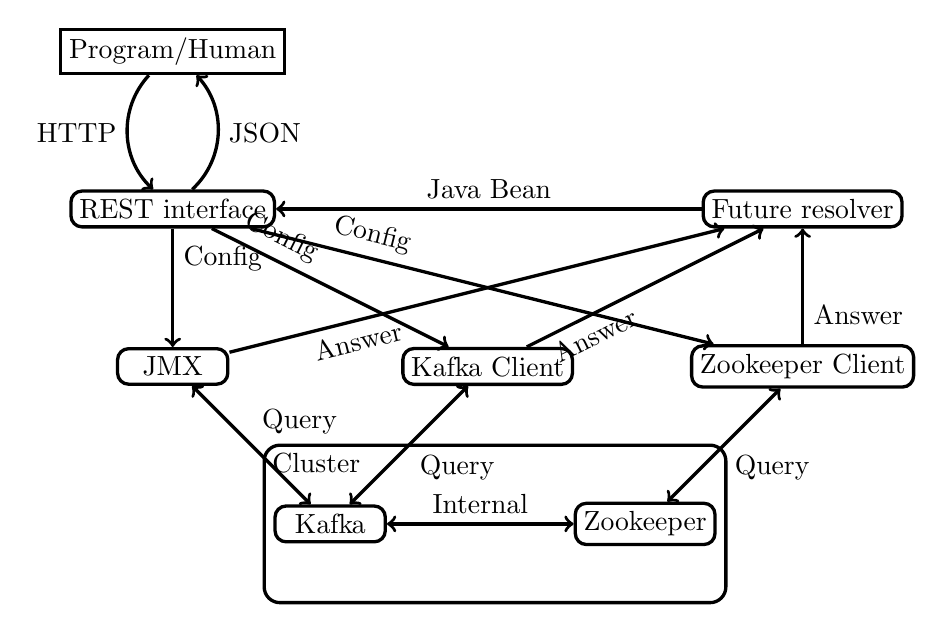
\begin{tikzpicture}[ % has a lot of options; consult the pgf manual
bend angle=45,
long_square/.style={rectangle, draw=black, fill=white, very thick, inner sep=3pt, minimum width=14mm},
rounded_square/.style={rectangle, rounded corners, draw=black, fill=white, very thick, inner sep=3pt, minimum width=14mm},
empty_circle/.style={rectangle, rounded corners=2mm, draw=black, fill=white, very thick, minimum size=4mm},
point/.style={circle, inner sep=0mm},
fit_square/.style={rectangle, rounded corners=2mm, draw=black, very thick, minimum height=20mm},
both_arrow/.style={<->, very thick},
out_arrow/.style={->, very thick},
out_hollow_arrow/.style={-open triangle 90, very thick},
in_arrow/.style={<-, very thick},
dashed_line/.style={loosely dashed, very thick},
above_edge_text/.style={above, midway, sloped}
]

% \node[type](name_of_node)[above/below/right/left/...=of name_of_node]{node_text}
%   edge[<->, bend left/right] node[auto, swap]{edge_text}(out_name_of_node)
% OR
% \node[type](name_of_node)[above/below/right/left/...=of name_of_node]{node_text}

\node[long_square](users) at (0,0) {Program/Human};

\node[rounded_square](REST_interface) at (0,-2) {REST interface};
\node[rounded_square](future_resolver) at (8,-2) {Future resolver};

\node[rounded_square](jmx) at (0,-4) {JMX};
\node[rounded_square](kafka_client) at (4,-4) {Kafka Client};
\node[rounded_square](zookeeper_client) at (8,-4) {Zookeeper Client};

\node[rounded_square](kafka) at (2,-6) {Kafka};
\node[rounded_square](zookeeper) at (6,-6) {Zookeeper};



\node [fit_square, fit=(kafka) (zookeeper)] (cluster) {};
\node [anchor=north west] at (cluster.north west) {Cluster};

% \draw[->](name_of_node.direction) -- (name_of_node.direction)
% OR
% \draw[->](name_of_node.direction) to [bend right] node[]{edge_text} (name_of_node.direction)
% OR
% \draw[->](name_of_node.direction) .. controls +(up/down/right/left:10mm) and +(up/down/right/left:10mm) .. (name_of_node.direction);

\draw[out_arrow](users) to [bend right] node[auto,swap]{HTTP} (REST_interface);
\draw[out_arrow](REST_interface) to [bend right] node[auto,swap]{JSON} (users);

\draw[out_arrow](REST_interface) to [] node[auto,near start]{Config} (jmx);
\draw[out_arrow](REST_interface) to [] node[auto,near start,sloped]{Config} (kafka_client);
\draw[out_arrow](REST_interface) to [] node[auto,near start,sloped]{Config} (zookeeper_client);

\draw[out_arrow](future_resolver) to [] node[auto,swap]{Java Bean} (REST_interface);

\draw[out_arrow](jmx) to [] node[auto,swap,near start,sloped]{Answer} (future_resolver);
\draw[out_arrow](kafka_client) to [] node[auto,swap,near start,sloped]{Answer} (future_resolver);
\draw[out_arrow](zookeeper_client) to [] node[auto,swap,near start]{Answer} (future_resolver);

\draw[both_arrow](jmx) to [] node[auto]{Query} (kafka);
\draw[both_arrow](kafka_client) to [] node[auto]{Query} (kafka);
\draw[both_arrow](zookeeper_client) to [] node[auto]{Query} (zookeeper);

\draw[both_arrow](kafka) to [] node[auto]{Internal} (zookeeper);

\end{tikzpicture}

\end{document}